
\documentclass[a4paper, 12pt]{article}
\usepackage{geometry}
\geometry{margin=2cm}
\usepackage{graphicx} % Required for the inclusion of images
\usepackage[utf8]{inputenc}
%\usepackage{natbib} % Required to change bibliography style to APA
\usepackage{amsmath} % Required for some math elements 
\usepackage[spanish]{babel} 
%\usepackage{fontspec}
\usepackage{lineno,hyperref}
\usepackage{upgreek}
\usepackage{gensymb}
\usepackage{textcomp}
\usepackage{amssymb}
\usepackage{textgreek}
\usepackage{float}
\usepackage{fancyhdr}
\usepackage{dirtytalk}

\allowdisplaybreaks
%\textwidth18cm
%\textheight22cm
%\topmargin0cm
%\oddsidemargin2cm
%\hypersetup{hidelinks}

\usepackage{multirow}

\hypersetup{
    colorlinks=true,
    linkcolor=blue,
    }
\graphicspath{{img}}
\setlength\parindent{0pt} % Removes all indentation from paragraphs

\renewcommand{\labelenumi}{\alph{enumi}.} % Make numbering in the enumerate environment by letter rather than number (e.g. section 6)

\renewcommand{\b}{\textbf}

\newsavebox{\mygraphic}
\sbox{\mygraphic}{
\includegraphics[height=1cm]{logoUNRN.jpg}}


\pagestyle{fancy}

\fancyhead{}

\headheight 16pt

\fancyhead[LO]{\setlength{\unitlength}{1in}
	\begin{picture}(0,0)
		\put(0,0){\usebox{\mygraphic}}
	\end{picture}
	\hspace{1cm}
}

\fancyhead[CO] {\hspace{1.5cm} \large Física I: Ingenierías Ambiental, Electrónica y Telecomunicaciones}

%esto me pareció piola para enumerar los ejercicios
%lo saqué de acá: https://tex.stackexchange.com/questions/302948/numbered-exercises-as-sections
%%%%%%%%%%%%%%%%%%%%%%%%%%%%%%%%%%%%%%%%%5
\newcounter{eje}
\setcounter{eje}{0}
\newcounter{subeje}
\setcounter{subeje}{-1}
\renewcommand\thesubeje{\arabic{eje}\alph{subeje}}%
\newcommand \eje{%
  \vspace{.2cm}
  \par\noindent
  \ifnum\value{subeje}>-1
    \refstepcounter{subeje}%
    \llap{\thesubeje)\quad}%
  \else
    \refstepcounter{eje}%
    \llap{\theeje)\quad}%
  \fi
}
\begin{document}
\pagestyle{fancy}

\begin{center}

	{\Large \textbf{Primer parcial}}
 
\vspace{.2cm}

{viernes 8/9}
\end{center}


\eje{\bf Velocidad relativa}  Un piloto desea que su aeronave vuele en dirección norte respecto del suelo, pero pero viento de 60.0 km/hr sopla desde el oeste.
a) Si la velocidad del avión con respellcto al viento es de 320.0 km/hr, ¿hacia dónde debe dirigir
el avión el piloto para lograrlo?
b) ¿Cuál es la velocidad del avión respecto del suelo?
c) Muestre en un gráfico los vectores velocidad involucrados en sus cálculos.


\eje{\bf Cinemática} Una persona lanza un palito a 30 km/hr con un ángulo de 45$\degree$ respecto de la horizontal.
Simuláneamente el perro galgo, que se encontraba a su lado, corre a buscarlo partiendo desde el reposo, acelerando de manera constante hasta que lo toma.
Encuentre el valor de la aceleración del perrito, y la velocidad del animal cuando toma el palito. Suponga que el la altura de a la que se lanza el palito y el perro lo recibe es la misma.


\eje{\bf Estática} Dos cajas están conectadas por una polea como se muestra en la figura. ¿Cuál es la fuerza \b F
máxima que puede ejercerse sobre la caja de arriba sin que deslicen entre sí ? La caja A tiene masa mA = 2 kg, la caja B tiene masa mB = 3 kg y el coeficiente de roce estático entre ambas es 0.5. Considere que entre la caja B y la mesa no hay rozamiento.


\begin{figure}[H]
\begin{center}
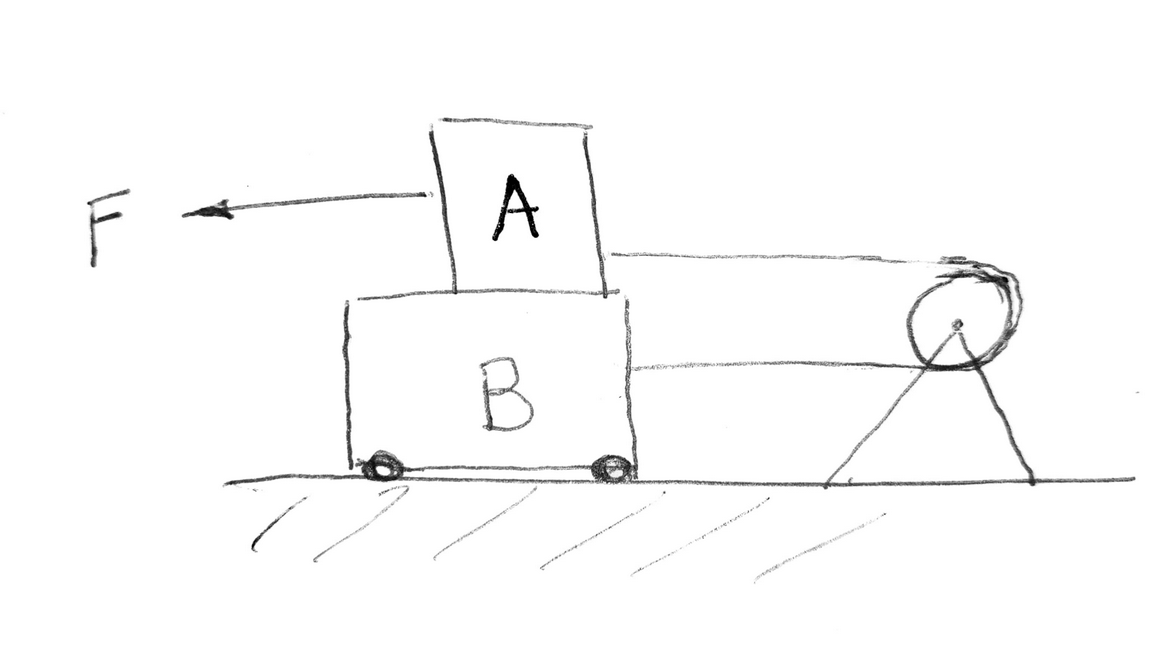
\includegraphics[clip,width = .45\columnwidth]{parcial2023_estatica}
\end{center}
\end{figure}

\eje{\bf Dinámica} El bloque con forma de cuña de la figura se acelera de tal manera que el carrito no desliza por la pendiente, ni para arriba, ni para abajo. Despreciando el rozamiento, encontrar la aceleración de la cuña para que esto ocurra

\begin{figure}[H]
\begin{center}
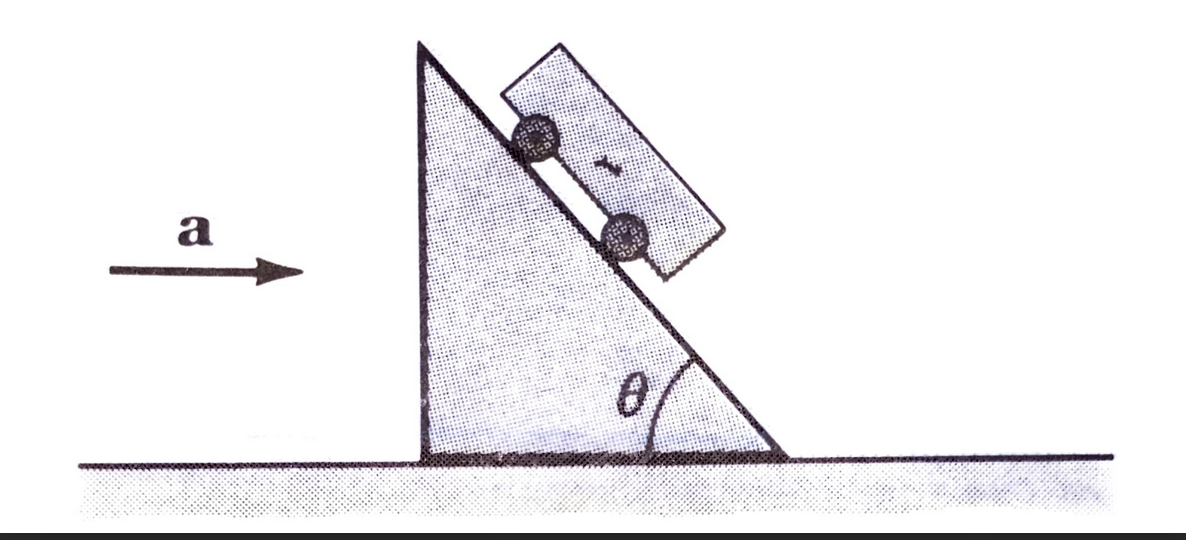
\includegraphics[clip,width = .45\columnwidth]{parcial2023_dinamica}
\end{center}
\end{figure}

\end{document}